\chapter{Szenarien im Ampelbereich}
Aus Abbildung \ref{fig:szenarien} ergeben sich folgende Szenarien: 
\begin{figure}[H]  
    \centering  
    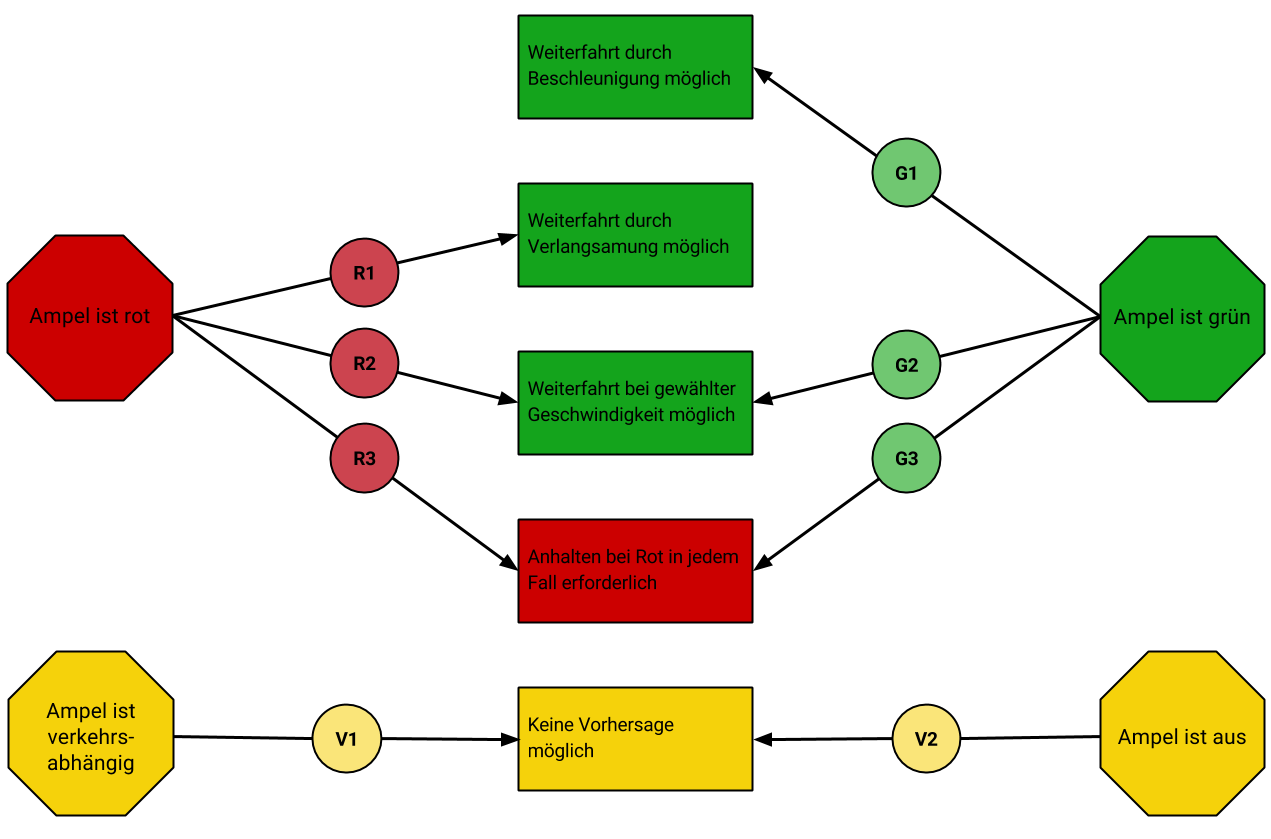
\includegraphics[width=1\textwidth]{Szenarien} 
    \caption[Szenarien]{Szenarien im Ampelbereich}
    \label{fig:szenarien}
\end{figure}
\paragraph{Szenario 1:} 
Die Ampelschaltung erlaubt momentan kein reibungsloses Passieren. 
\paragraph{Szenario 2: Konstante Weiterfahrt möglich} 
Ist die empfohlene Geschwindigkeit gleich der aktuellen, ist ein reibungsloses Passieren bei beibehaltenem Tempo möglich. Es besteht kein Handlungsbedarf. 
\paragraph{Szenario 3: Reibungsloses Passieren durch Beschleunigung möglich} 
Zeigt die Ampel im Moment Grün und ist die empfohlene Geschwindigkeit höher als die aktuelle, ist ein reibungsloses Passieren durch Beschleunigung zu erreichen. Bei der Anzeige der Progressionsgeschwindigkeit ist selbstverständlich die geltende Höchstgeschwindigkeitsbegrenzung zu beachten. 
\paragraph{Szenario 4: Reibungsloses Passieren duch Verlangsamen möglich} 
Zeigt die Ampel im Moment Rot und ist die empfohlene Geschwindigkeit niedriger als die aktuelle, ist ein reibungsloses Passieren durch Verlangsamung zu erreichen.
\paragraph{Szenario 5: Reibungsloses Passieren durch Beschleunigung möglich} 
Zeigt die Ampel im Moment Grün und ist die empfohlene Geschwindigkeit höher als die aktuelle, ist ein reibungsloses Passieren durch Beschleunigung zu erreichen. Bei der Anzeige der Progressionsgeschwindigkeit ist selbstverständlich die geltende Höchstgeschwindigkeitsbegrenzung zu beachten. 
\paragraph{Szenario 6: Reibungsloses Passieren duch Verlangsamen möglich} 
Zeigt die Ampel im Moment Rot und ist die empfohlene Geschwindigkeit niedriger als die aktuelle, ist ein reibungsloses Passieren durch Verlangsamung zu erreichen.
